\chapter{Desenvolvimento} \label{desenvolvimento}
\section{Métodos}
Pesquisa feita em sites como "https://sullygnome.com" e dados coletados manualmente e transcritos para um arquivo .csv para utlização em um programa em python aonde esses dados são transformados em gráficos interativos.

Esse programa em python utliza da biblioteca plotly para fazer os graficos da biblioteca  
tkinter para criar botões parar selecionar quais graficos serem formados e da biblioteca pandas para transformar os dados dos arquivos .csv em um variavel com todos os dados necessarios para a "plotagem" do gráfico.

As funções utilizadas da biblioteca plotly foram: .Bar(), para tranformar o dados em um grafico de barras, .Pie(), para transformar em um grafico de pizza, iplot(), que cria em um servidor local o visualizador desses graficos, e .head(), que limita a quantidade de dados a serem observados no gráfico. 

Docmentação e informações no site da biblioteca https://plotly.com.

As funções utilizadas da biblioteca pandas foram: .read\textunderscore csv(), lê os dados em um arquivo .csv,e .apply() e .to\textunderscore numeric, para tranformar os dados em valores númericos entendiveis pela lingaguem. Docmentação e informações no site da biblioteca https://plotly.com. 

Docmentação e informações no site da biblioteca https://pandas.pydata.org

As funções utilizadas da biblioteca tkinter foram: Tk(), que cria a base aonde os botões de seleção são criados, Button(), que cria botões individuais para diversas funções, .pack(), que campacta esses blocos na base, e .mainloop(), que abre e roda os botões até que a janela seja fechada pelo utilizador. 

Docmentação e informações no site da biblioteca https://docs.python.org/3/library/tkinter.html

\usepackage{graphicx}
\usepackage[portuguese]{babel} % Para termos legendas em português
\date{} % para este exemplo, deixarei a data vazia
 
\begin{figure}[h]
\caption{Bibliotecas}
 
\centering % para centralizarmos a figura
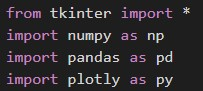
\includegraphics[width=5cm]{Figuras/Bibliotecas.jpg} % leia abaixo
\label{figura:qualquernome}
\end{figure}
 
Na Fig. \ref{figura:qualquernome}, Import das bibliotecas em python
\section{Resultados}

Com a coleta de dados e a demonstração grafica dos mesmos, foi possivel visualizar nitidademente diferenças entre os mesmes iniciais da plataforma, o periodo pre pandemia e o pos pandemia, sendo que os maiores valores são os pos pandemia por uma procura maior por esse tipo de entretenimento virtual.

\begin{figure}[h]
\caption{Tempo em horas}
 
\centering % para centralizarmos a figura
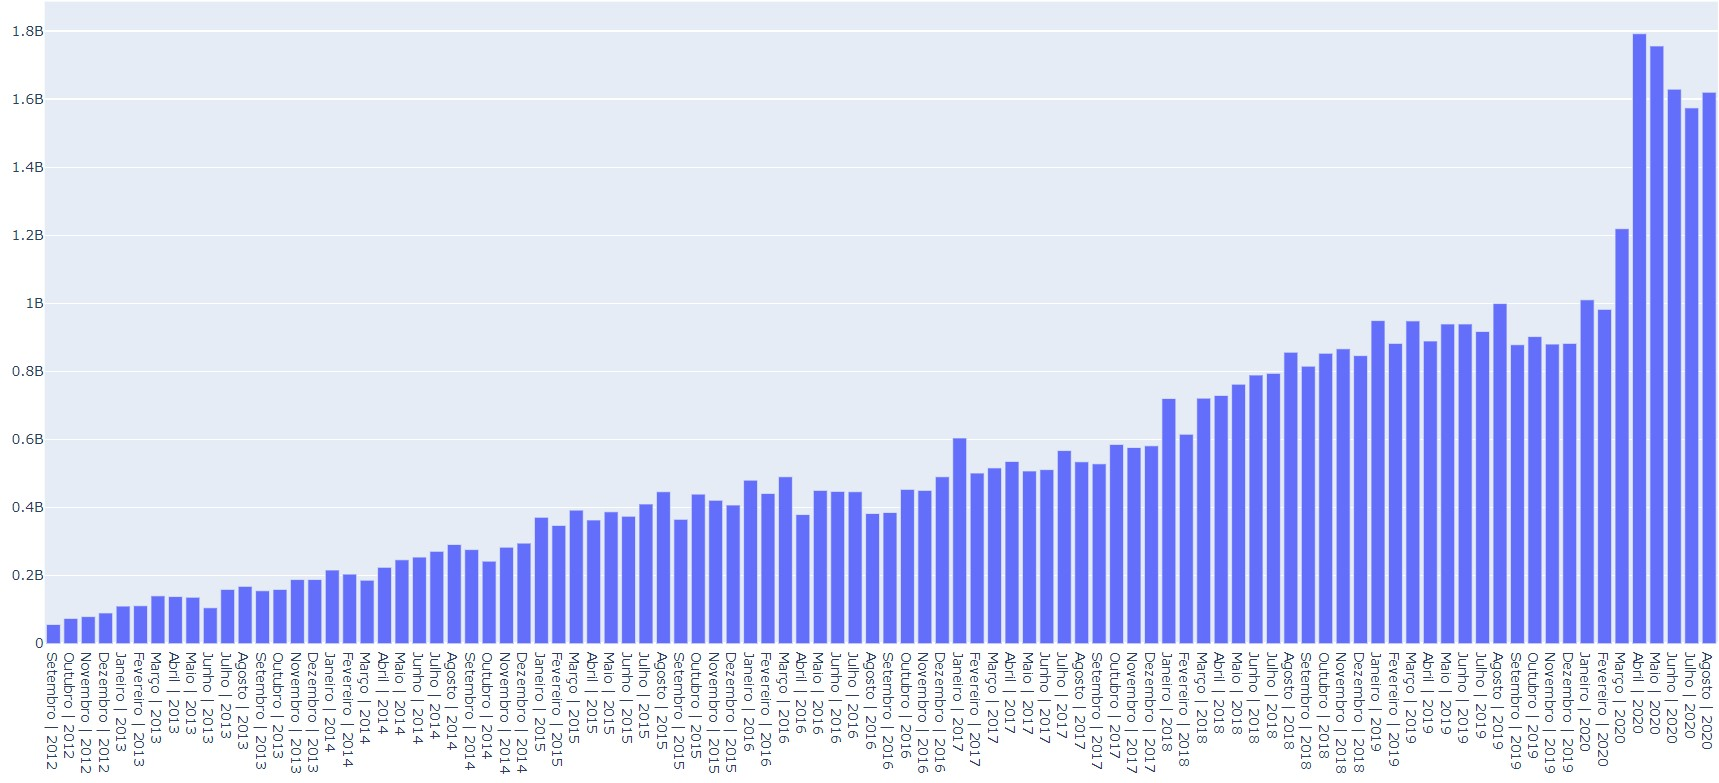
\includegraphics[width=17cm]{Figuras/Tempo_horas.jpg} % leia abaixo
\label{figura:qualquernome}
\end{figure}
Na Fig. \ref{figura:qualquernome}, Grafico em barras do tempo em horas assistido na plataforma

Além disso, é possivel visualizar também a diferença entre quais eram as categorias mais pesquisadas e acessadas no passado e agora, com uma crescente vindo do "just chatting"  desde que se começou a pandemia e alguns sucessos de momento como no caso do "valorant".

\begin{figure}[h]
\caption{Categorias em horas}
 
\centering % para centralizarmos a figura
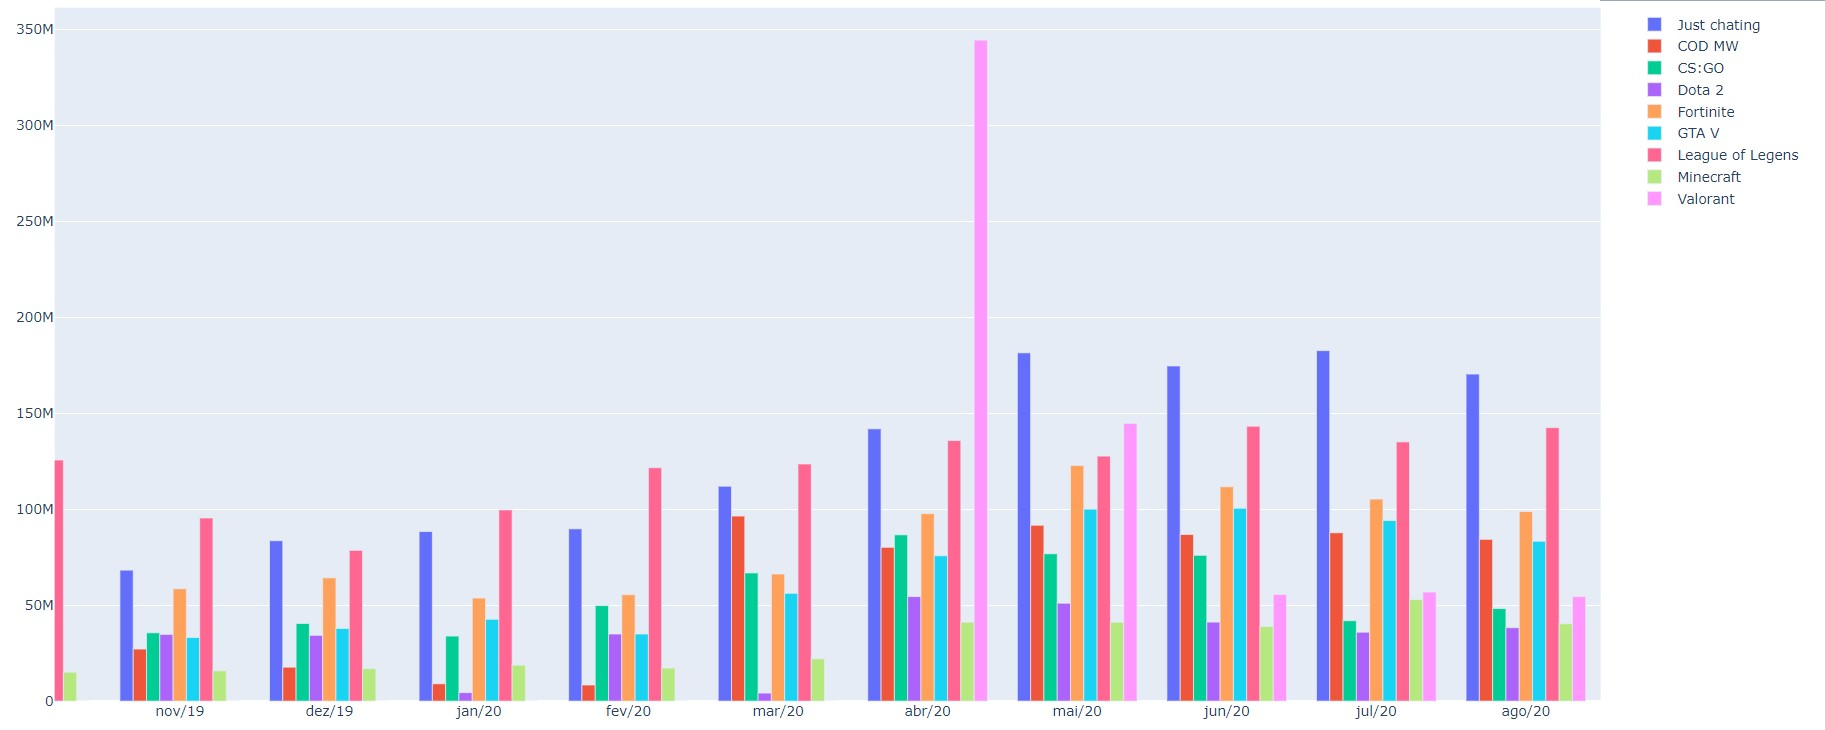
\includegraphics[width=15cm]{Figuras/Categorias_1.jpg} % leia abaixo
\label{figura:qualquernome}
\end{figure}
Na Fig. \ref{figura:qualquernome}, Grafico em barras do tempo em horas assistido das categorias na plataforma

